\documentclass[11pt,a4paper]{article}

% ==========================================
% PACKAGES & TYPOGRAPHY
% ==========================================
\usepackage[utf8]{inputenc}
\usepackage[english]{babel}
\usepackage[T1]{fontenc}
\usepackage{charter}
\usepackage[scaled=0.88]{helvet}
\usepackage{courier}
\usepackage[a4paper,top=1.6cm,bottom=1.6cm,left=1.7cm,right=1.7cm,headheight=14pt]{geometry}
\usepackage{amsmath,amssymb}
\usepackage{booktabs,tabularx,multirow}
\usepackage{graphicx}
\usepackage{xcolor}
\usepackage{enumitem}
\usepackage{float}
\usepackage{fancyhdr}
\usepackage{titlesec}
\usepackage{tikz}
\usetikzlibrary{arrows.meta,positioning,calc,shapes.geometric}
\usepackage{microtype}
\usepackage[hidelinks,colorlinks=true,linkcolor=primaryblue,citecolor=accentteal,urlcolor=primaryblue]{hyperref}

% ==========================================
% PROFESSIONAL PALETTE
% ==========================================
\definecolor{primaryblue}{RGB}{18, 48, 92}
\definecolor{accentteal}{RGB}{24, 108, 142}
\definecolor{darkcharcoal}{RGB}{40, 50, 65}
\definecolor{bordergray}{RGB}{218, 226, 236}
\definecolor{subtlegray}{RGB}{247, 249, 252}
\definecolor{badgeblue}{RGB}{232, 241, 250}
\definecolor{badgeteal}{RGB}{226, 244, 244}

% ==========================================
% HEADER & FOOTER
% ==========================================
\pagestyle{fancy}
\fancyhf{}
\fancyhead[L]{\small\color{darkcharcoal}\textsc{TripMate AI} --- Technical Project Proposal}
\fancyhead[R]{\small\color{accentteal}\textbf{Unified AI Agent \& Cloud Architecture}}
\fancyfoot[L]{\small\color{gray}Group Project Technical Proposal}
\fancyfoot[R]{\small\color{darkcharcoal}\thepage}
\renewcommand{\headrulewidth}{0.5pt}
\renewcommand{\footrulewidth}{0.3pt}

% ==========================================
% TYPOGRAPHY & SECTION FORMATTING (NO GAPS)
% ==========================================
\raggedbottom
\setlength{\parindent}{0pt}
\setlength{\parskip}{2.2pt plus 0.4pt minus 0.4pt}
\linespread{1.03}

\titleformat{\section}
{\Large\bfseries\color{primaryblue}}{\thesection.}{0.5em}{}[\vspace{1pt}{\color{accentteal!40}\titlerule[0.8pt]}]
\titleformat{\subsection}
{\large\bfseries\color{accentteal}}{\thesubsection.}{0.5em}{}
\titleformat{\subsubsection}
{\normalsize\bfseries\color{darkcharcoal}}{\thesubsubsection.}{0.4em}{}
\titlespacing*{\section}{0pt}{5pt plus 1pt minus 1pt}{2pt plus 0.5pt minus 0.5pt}
\titlespacing*{\subsection}{0pt}{3.5pt plus 1pt minus 1pt}{1.5pt plus 0.5pt minus 0.5pt}
\titlespacing*{\subsubsection}{0pt}{2.5pt plus 0.5pt minus 0.5pt}{1pt}
\setlist[itemize]{noitemsep,topsep=1pt,parsep=0pt,partopsep=0pt,leftmargin=1.2em}
\setlist[enumerate]{noitemsep,topsep=1pt,parsep=0pt,partopsep=0pt,leftmargin=1.2em}

% Tighten float spacing to eliminate whitespace gaps
\setlength{\floatsep}{4pt plus 1pt minus 1pt}
\setlength{\textfloatsep}{5pt plus 1pt minus 1pt}
\setlength{\intextsep}{4pt plus 1pt minus 1pt}

\begin{document}

% ==========================================
% PAGE 1: OVERVIEW, PROBLEM, SCOPE, LIFECYCLE & PLATFORM FEATURES
% ==========================================
\begin{center}
{\LARGE\bfseries\color{primaryblue} TripMate AI: Intelligent Group Activity \& Travel Planning Platform}\\[0.10cm]
{\large\bfseries\color{accentteal} Unified AI Agent Architecture, Cloud Deployment \& Production Engineering}\\[0.14cm]
{\small\textbf{Technical Project Proposal for Academic Supervisor} \quad$\vert$\quad \textbf{Group Project Concept}}\\[0.08cm]
\rule{\textwidth}{0.8pt}\\[0.08cm]
{\footnotesize \textbf{Project Team (6 Members):} Ta Quang Huy \quad Ha Dang Huy \quad Pham Dinh Anh Duong \quad Nguyen Minh Duc \quad Nguyen Tung Duong \quad Dinh Tien Luan}
\end{center}
\vspace{-0.15cm}

\section{Introduction, Scope \& Product Overview}

\subsection{The Problem: Pain Points in Group Trip Planning}
Coordinating leisure outings or vacations with friends is notoriously friction-heavy:
\begin{itemize}
\item \textbf{Tool Fragmentation:} Planning requires juggling 5+ disconnected applications (Google Maps, review blogs, Agoda, Booking.com, chat apps).
\item \textbf{Preference Deadlocks:} Conflicting budgets, dietary restrictions, and activity styles stall decision-making.
\item \textbf{Organizer Burnout \& Buried Context:} Chat polls and venue links quickly get buried under hundreds of messages, leaving a single person overwhelmed with building and adjusting schedules.
\end{itemize}

\subsection{Target Users \& Practical Scope}
\label{sec:target_audience}
\begin{itemize}
\item \textbf{Target Users:} Small groups (2--10 friends, university students, coworkers) organizing weekend city hangouts or multi-day vacations.
\item \textbf{Practical Scope:} Domestic travel in Vietnam and visa-free ASEAN destinations, focusing strictly on intelligent scheduling, venue optimization, and real-time collaboration without visa complexities.
\end{itemize}

\subsection{The Solution: Two-Stage Consensus Planning Flow}
TripMate AI unifies group planning through a collaborative room powered by a \textbf{single, unified AI Agent (DeepSeek-V4)} that guides the group through two consensus checkpoints (Figure~\ref{fig:lifecycle}):
\begin{enumerate}
\item \textbf{Desires Capture:} Members share dates, budgets, and vibes in persistent room chat, saved directly into PostgreSQL.
\item \textbf{Macro Consensus:} The AI drafts high-level dates and daily themes; the group discusses and votes to lock the roadmap.
\item \textbf{Micro Curation \& Stop Voting:} The AI queries live APIs (Google Places, Agoda, Klook) to populate venues clustered within a 2--3\,km radius per half-day block. Members vote thumbs UP/DOWN, with 1-click alternative swaps.
\item \textbf{Final Confirmation:} The Host confirms the finalized plan, generating PDF and calendar (.ics) exports with synchronized Mapbox routes.
\end{enumerate}

\begin{figure}[H]
\centering
\resizebox{0.96\textwidth}{!}{
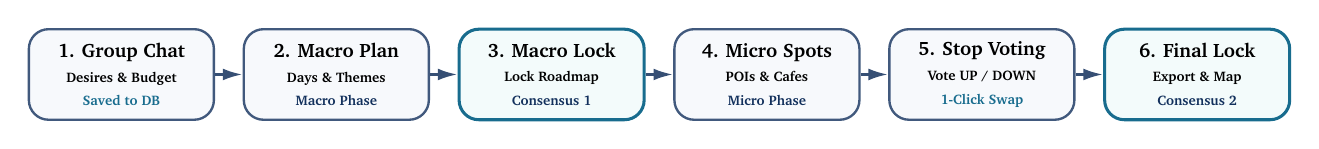
\begin{tikzpicture}[
  node distance=0.35cm,
  stepbox/.style={rectangle, draw=primaryblue!80, fill=subtlegray, rounded corners=2.5mm, line width=0.85pt, minimum width=2.35cm, minimum height=1.15cm, align=center, font=\scriptsize\bfseries},
  lockbox/.style={rectangle, draw=accentteal, fill=badgeteal!40!white, rounded corners=2.5mm, line width=1.1pt, minimum width=2.35cm, minimum height=1.15cm, align=center, font=\scriptsize\bfseries},
  flow/.style={-{Latex[length=2.5mm,width=1.5mm]}, line width=1pt, color=primaryblue!85}
]
\node[stepbox] (s1) {1. Group Chat\\[0.03cm]{\tiny Desires \& Budget}\\[0.02cm]{\tiny\color{accentteal}Saved to DB}};
\node[stepbox, right=of s1] (s2) {2. Macro Plan\\[0.03cm]{\tiny Days \& Themes}\\[0.02cm]{\tiny\color{primaryblue}Macro Phase}};
\node[lockbox, right=of s2] (s3) {3. Macro Lock\\[0.03cm]{\tiny Lock Roadmap}\\[0.02cm]{\tiny\color{primaryblue}\textbf{Consensus 1}}};
\node[stepbox, right=of s3] (s4) {4. Micro Spots\\[0.03cm]{\tiny POIs \& Cafes}\\[0.02cm]{\tiny\color{primaryblue}Micro Phase}};
\node[stepbox, right=of s4] (s5) {5. Stop Voting\\[0.03cm]{\tiny Vote UP / DOWN}\\[0.02cm]{\tiny\color{accentteal}1-Click Swap}};
\node[lockbox, right=of s5] (s6) {6. Final Lock\\[0.03cm]{\tiny Export \& Map}\\[0.02cm]{\tiny\color{primaryblue}\textbf{Consensus 2}}};

\draw[flow] (s1) -- (s2);
\draw[flow] (s2) -- (s3);
\draw[flow] (s3) -- (s4);
\draw[flow] (s4) -- (s5);
\draw[flow] (s5) -- (s6);
\end{tikzpicture}
}
\vspace{-0.25cm}
\caption{Two-stage consensus planning flow: gather desires $\rightarrow$ macro roadmap $\rightarrow$ lock macro $\rightarrow$ curate micro spots $\rightarrow$ granular vote $\rightarrow$ final plan lock}
\label{fig:lifecycle}
\end{figure}

\section{Platform Features \& User Experience}

\subsection{Dual Planning Scopes}
\begin{itemize}
\item \textbf{Day Hangouts:} Rapid curation for spontaneous outings (e.g., \textit{``cafe $\rightarrow$ board game lounge $\rightarrow$ hotpot''}), prioritizing currently open venues with minimal transit times.
\item \textbf{Multi-Day Vacations:} Complete travel itineraries (e.g., \textit{``4 days in Da Nang \& Hoi An''}) combining hotel recommendations, daily meal spots, sights, and optimized routes.
\end{itemize}

\subsection{Shared Collaborative Room \& Live Map Canvas}
\begin{itemize}
\item \textbf{Invite via Link \& Role Access:} Instant room entry with \textit{Host} (plan locking, settings) and \textit{Member} (chat, stop voting, swaps) permissions.
\item \textbf{Interactive Timeline \& Mapbox GL:} Draggable stop cards displaying photos, opening hours, estimated stay duration, and live Mapbox route navigation.
\end{itemize}

\subsection{Two-Tier Consensus Engine}
\label{sec:consensus}
\begin{itemize}
\item \textbf{Stage 1 (Macro Approval):} Group locks the high-level roadmap before any expensive venue API calls are triggered.
\item \textbf{Stage 2 (Micro Stop Voting):} Individual stops are voted UP/DOWN. Downvoted venues immediately present 2 pre-fetched backup options with 1-click swaps.
\item \textbf{Living Itinerary:} Final plan confirmation persists normalized records to PostgreSQL but leaves the itinerary dynamic for real-time on-trip adjustments.
\end{itemize}

\clearpage
% ==========================================
% PAGE 2: THE AI AGENT: ARCHITECTURE, DATA PIPELINE & ACTIVITY DIAGRAM
% ==========================================
\section{The AI Agent: Architecture, Workflow \& Grounding Pipeline}

\subsection{Unified AI Agent: DeepSeek-V4 with Two-Phase State Execution}
TripMate AI utilizes a \textbf{single, unified AI Agent powered by DeepSeek-V4} in LangGraph. To resolve latency bottlenecks and ensure clean testability, the agent operates in two decoupled state phases:
\begin{itemize}
\item \textbf{Phase 1 (Macro Planning State):} Proposes dates, pacing, and daily themes without invoking external travel APIs, conserving tokens until macro consensus is reached.
\item \textbf{Phase 2 (Micro Curation State):} Activated only after macro approval. Executes external tool calls, applies 2--3\,km geo-clustering to prevent zigzag routes, and prepares alternative stops.
\item \textbf{Model Abstraction Layer:} Built using LangChain/LangGraph model abstractions. DeepSeek-V4 serves as the primary reasoning engine, with transparent fallback to OpenAI (GPT-4o), Anthropic Claude, or Google Gemini to prevent vendor lock-in.
\item \textbf{Typed State Persistence:} Checkpoints of \texttt{AgentState} are saved in PostgreSQL via \texttt{AsyncPostgresSaver} through an authenticated Data Access Layer (DAL).
\end{itemize}

\subsection{AI Agent Data Pipeline}
\label{sec:agent_integration}
Figure~\ref{fig:agent_data_flow} illustrates the unified AI agent state and data pipeline, connecting room context, two-phase LangGraph states, typed checkpoints, model abstraction, and resilient tooling:

\begin{figure}[H]
\centering
\resizebox{0.92\textwidth}{!}{
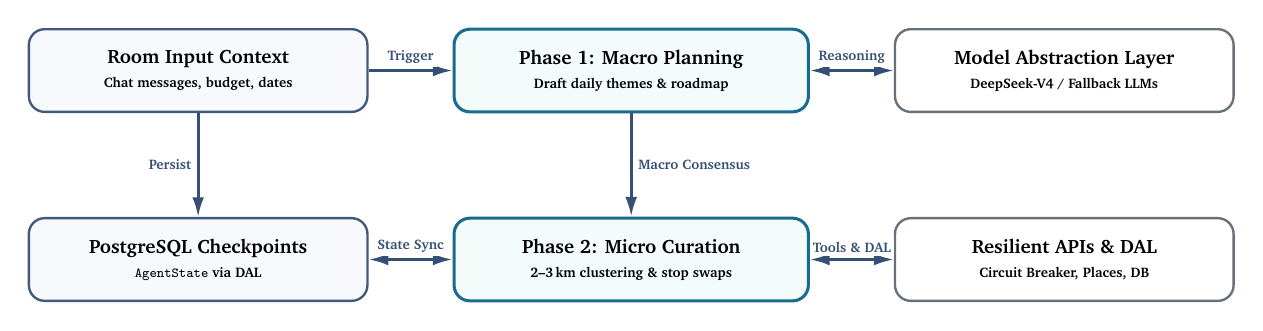
\begin{tikzpicture}[
  box/.style={rectangle, draw=primaryblue!80, fill=subtlegray, rounded corners=2mm, line width=0.85pt, minimum width=4.3cm, minimum height=1.05cm, align=center, font=\scriptsize\bfseries},
  agentbox/.style={rectangle, draw=accentteal, fill=badgeteal!40!white, rounded corners=2mm, line width=1.1pt, minimum width=4.5cm, minimum height=1.05cm, align=center, font=\scriptsize\bfseries},
  tool/.style={rectangle, draw=darkcharcoal!70, fill=white, rounded corners=2mm, line width=0.85pt, minimum width=4.3cm, minimum height=1.05cm, align=center, font=\scriptsize\bfseries},
  flow/.style={-{Latex[length=2.5mm,width=1.5mm]}, line width=1pt, color=primaryblue!85},
  biflow/.style={{Latex[length=2.5mm,width=1.5mm]}-{Latex[length=2.5mm,width=1.5mm]}, line width=1pt, color=primaryblue!85}
]

% Row 1: Macro Flow (y = 1.2)
\node[box] (input) at (0, 1.2) {\textbf{Room Input Context}\\[0.02cm]{\tiny Chat messages, budget, dates}};
\node[agentbox] (macro) at (5.5, 1.2) {\textbf{Phase 1: Macro Planning}\\[0.02cm]{\tiny Draft daily themes \& roadmap}};
\node[tool] (llm) at (11.0, 1.2) {\textbf{Model Abstraction Layer}\\[0.02cm]{\tiny DeepSeek-V4 / Fallback LLMs}};

% Row 2: Micro Flow (y = -1.2)
\node[box] (state) at (0, -1.2) {\textbf{PostgreSQL Checkpoints}\\[0.02cm]{\tiny \texttt{AgentState} via DAL}};
\node[agentbox] (micro) at (5.5, -1.2) {\textbf{Phase 2: Micro Curation}\\[0.02cm]{\tiny 2--3\,km clustering \& stop swaps}};
\node[tool] (tools) at (11.0, -1.2) {\textbf{Resilient APIs \& DAL}\\[0.02cm]{\tiny Circuit Breaker, Places, DB}};

% Clean Orthogonal Connections
\draw[flow] (input) -- node[above=0.03cm,font=\tiny\bfseries,fill=white,inner sep=1.2pt]{Trigger} (macro);
\draw[biflow] (macro) -- node[above=0.03cm,font=\tiny\bfseries,fill=white,inner sep=1.2pt]{Reasoning} (llm);

\draw[flow] (input) -- node[left=0.03cm,font=\tiny\bfseries,fill=white,inner sep=1.2pt]{Persist} (state);
\draw[flow] (macro) -- node[right=0.03cm,font=\tiny\bfseries\color{accentteal},fill=white,inner sep=1.2pt]{Macro Consensus} (micro);

\draw[biflow] (state) -- node[above=0.03cm,font=\tiny\bfseries,fill=white,inner sep=1.2pt]{State Sync} (micro);
\draw[biflow] (micro) -- node[above=0.03cm,font=\tiny\bfseries,fill=white,inner sep=1.2pt]{Tools \& DAL} (tools);

\end{tikzpicture}
}
\vspace{-0.25cm}
\caption{AI Agent state and data pipeline: two-phase LangGraph state execution with model abstraction and resilient tooling}
\label{fig:agent_data_flow}
\end{figure}

\subsection{Group Planning Workflow: Activity Diagram}
\label{sec:workflow_steps}
Figure~\ref{fig:activity_diagram} illustrates the end-to-end user and AI interaction flow across two streamlined swimlanes:

\begin{figure}[H]
\centering
\resizebox{0.78\textwidth}{!}{
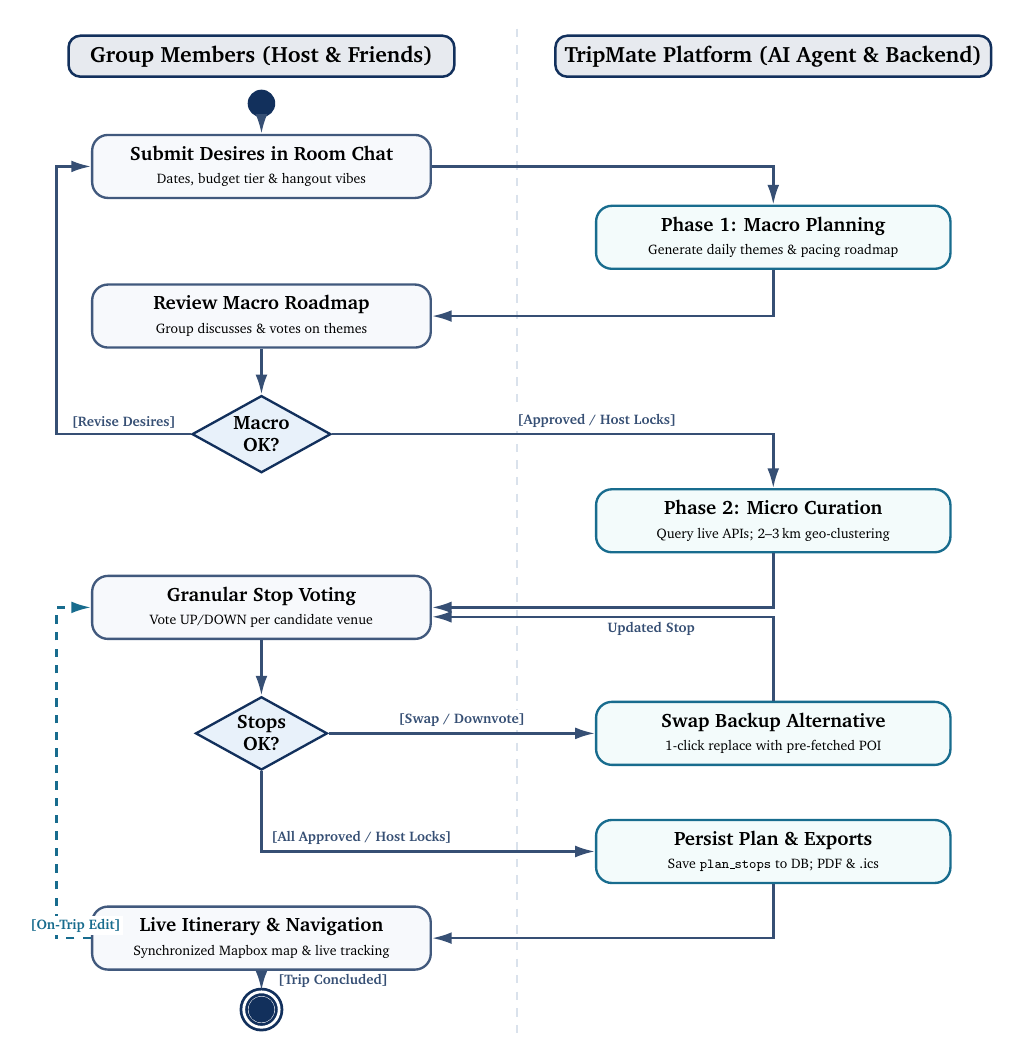
\begin{tikzpicture}[
  userbox/.style={rectangle, draw=primaryblue!80, fill=subtlegray, rounded corners=2mm, line width=0.85pt, minimum width=4.3cm, minimum height=0.80cm, align=center, font=\scriptsize},
  aibox/.style={rectangle, draw=accentteal, fill=badgeteal!40!white, rounded corners=2mm, line width=0.85pt, minimum width=4.5cm, minimum height=0.80cm, align=center, font=\scriptsize},
  decision/.style={diamond, aspect=1.8, draw=primaryblue, fill=badgeblue, line width=0.85pt, align=center, font=\scriptsize\bfseries, inner sep=1.2pt},
  lanehdr/.style={rectangle, draw=primaryblue, fill=primaryblue!10!white, rounded corners=1.5mm, line width=0.9pt, minimum width=4.9cm, minimum height=0.52cm, align=center, font=\footnotesize\bfseries},
  actarrow/.style={-{Latex[length=2.5mm,width=1.5mm]}, line width=0.9pt, color=primaryblue!85}
]

% 2 Wide Swimlanes
\node[lanehdr] (h1) at (0, 0) {Group Members (Host \& Friends)};
\node[lanehdr] (h2) at (6.5, 0) {TripMate Platform (AI Agent \& Backend)};

% Central Dividing Line
\draw[dashed, color=bordergray, line width=0.7pt] (3.25, 0.35) -- (3.25, -12.4);

% 1. Start & Preferences
\node[circle, fill=primaryblue, minimum size=3.5mm] (start) at (0, -0.6) {};
\node[userbox] (act1) at (0, -1.4) {\textbf{Submit Desires in Room Chat}\\[0.02cm]{\tiny Dates, budget tier \& hangout vibes}};
\draw[actarrow] (start) -- (act1);

% 2. Phase 1: Macro Planning
\node[aibox] (act2) at (6.5, -2.3) {\textbf{Phase 1: Macro Planning}\\[0.02cm]{\tiny Generate daily themes \& pacing roadmap}};
\draw[actarrow] (act1.east) -| (act2.north);

% 3. Review Macro Plan
\node[userbox] (act3) at (0, -3.3) {\textbf{Review Macro Roadmap}\\[0.02cm]{\tiny Group discusses \& votes on themes}};
\draw[actarrow] (act2.south) |- (act3.east);

% 4. Decision 1: Macro OK?
\node[decision] (dec1) at (0, -4.8) {Macro\\OK?};
\draw[actarrow] (act3.south) -- (dec1.north);

% Loopback [Revise Desires]
\draw[actarrow] (dec1.west) -- (-2.6, -4.8) node[above=0.02cm,pos=0.5,font=\tiny\bfseries\color{primaryblue},fill=white,inner sep=1pt]{[Revise Desires]} |- (act1.west);

% 5. Phase 2: Micro Curation
\node[aibox] (act4) at (6.5, -5.9) {\textbf{Phase 2: Micro Curation}\\[0.02cm]{\tiny Query live APIs; 2--3\,km geo-clustering}};
\draw[actarrow] (dec1.east) -| node[above=0.03cm,pos=0.3,font=\tiny\bfseries\color{accentteal},fill=white,inner sep=1.2pt]{[Approved / Host Locks]} (act4.north);

% 6. Stop Voting
\node[userbox] (act5) at (0, -7.0) {\textbf{Granular Stop Voting}\\[0.02cm]{\tiny Vote UP/DOWN per candidate venue}};
\draw[actarrow] (act4.south) |- (act5.east);

% 7. Decision 2: Stops OK?
\node[decision] (dec2) at (0, -8.6) {Stops\\OK?};
\draw[actarrow] (act5.south) -- (dec2.north);

% 1-Click Swap Alternative POI
\node[aibox] (act_swap) at (6.5, -8.6) {\textbf{Swap Backup Alternative}\\[0.02cm]{\tiny 1-click replace with pre-fetched POI}};
\draw[actarrow] (dec2.east) -- node[above=0.03cm,font=\tiny\bfseries\color{primaryblue},fill=white,inner sep=1.2pt]{[Swap / Downvote]} (act_swap.west);
\draw[actarrow] (act_swap.north) |- node[below right=0.02cm,pos=0.75,font=\tiny\bfseries\color{accentteal},fill=white,inner sep=1pt]{Updated Stop} ($(act5.east)+(0,-0.12)$);

% 8. Persist & Exports
\node[aibox] (act6) at (6.5, -10.1) {\textbf{Persist Plan \& Exports}\\[0.02cm]{\tiny Save \texttt{plan\_stops} to DB; PDF \& .ics}};
\draw[actarrow] (dec2.south) |- node[above=0.03cm,pos=0.65,font=\tiny\bfseries\color{accentteal},fill=white,inner sep=1.2pt]{[All Approved / Host Locks]} (act6.west);

% 9. Live Itinerary Navigation
\node[userbox] (act7) at (0, -11.2) {\textbf{Live Itinerary \& Navigation}\\[0.02cm]{\tiny Synchronized Mapbox map \& live tracking}};
\draw[actarrow] (act6.south) |- (act7.east);

% End Node
\node[circle, draw=primaryblue, line width=1pt, minimum size=4.5mm, double, double distance=1pt, below=0.25cm of act7] (end) {};
\node[circle, fill=primaryblue, minimum size=2.2mm] at (end) {};
\draw[actarrow] (act7.south) -- node[right=0.08cm,font=\tiny\bfseries\color{darkcharcoal}]{[Trip Concluded]} (end.north);

% Dynamic On-the-Go Adaptation Request
\draw[actarrow, dashed, color=accentteal] (act7.west) -- (-2.6, -11.2) node[above=0.02cm,pos=0.45,font=\tiny\bfseries\color{accentteal},fill=white,inner sep=1pt]{[On-Trip Edit]} |- (act5.west);

\end{tikzpicture}
}
\vspace{-0.25cm}
\caption{UML activity diagram: streamlined group planning workflow across user and AI system partitions}
\label{fig:activity_diagram}
\end{figure}

\clearpage
% ==========================================
% PAGE 3: AI GROUNDING PIPELINE, SYSTEM ARCHITECTURE, TECH STACK & CLOUD DEPLOYMENT
% ==========================================
\subsection{AI Reliability: Four-Tier Grounding Pipeline}
\label{sec:hallucination_mitigation}

To eliminate AI hallucinations (inventing fake places, closed venues, or unrealistic routes), TripMate AI verifies every recommendation through four simple steps (Figure~\ref{fig:hallucination_pipeline}):

\begin{figure}[H]
\centering
\resizebox{0.96\textwidth}{!}{
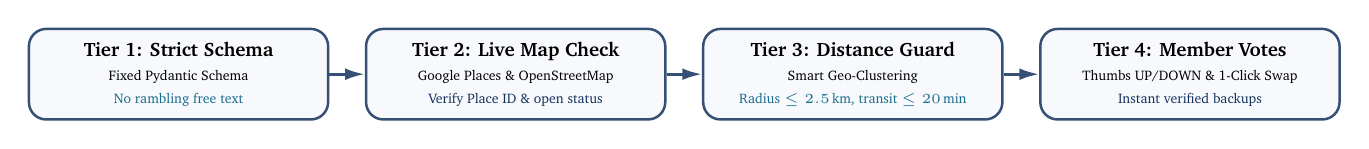
\begin{tikzpicture}[
  node distance=0.45cm,
  tierbox/.style={rectangle, draw=primaryblue!85, fill=subtlegray, rounded corners=2.2mm, line width=0.9pt, minimum width=3.8cm, minimum height=1.15cm, align=center, font=\scriptsize},
  arrow/.style={-{Latex[length=2.5mm,width=1.5mm]}, line width=1pt, color=primaryblue!85}
]
\node[tierbox] (t1) {\textbf{Tier 1: Strict Schema}\\[0.02cm]{\tiny Fixed Pydantic Schema}\\[0.01cm]{\tiny\color{accentteal}No rambling free text}};
\node[tierbox, right=of t1] (t2) {\textbf{Tier 2: Live Map Check}\\[0.02cm]{\tiny Google Places \& OpenStreetMap}\\[0.01cm]{\tiny\color{primaryblue}Verify Place ID \& open status}};
\node[tierbox, right=of t2] (t3) {\textbf{Tier 3: Distance Guard}\\[0.02cm]{\tiny Smart Geo-Clustering}\\[0.01cm]{\tiny\color{accentteal}Radius $\le 2.5$\,km, transit $\le 20$\,min}};
\node[tierbox, right=of t3] (t4) {\textbf{Tier 4: Member Votes}\\[0.02cm]{\tiny Thumbs UP/DOWN \& 1-Click Swap}\\[0.01cm]{\tiny\color{primaryblue}Instant verified backups}};

\draw[arrow] (t1) -- (t2);
\draw[arrow] (t2) -- (t3);
\draw[arrow] (t3) -- (t4);
\end{tikzpicture}
}
\vspace{-0.25cm}
\caption{TripMate AI four-tier live grounding and hallucination prevention pipeline}
\label{fig:hallucination_pipeline}
\end{figure}

\begin{itemize}[leftmargin=1.2em]
\item \textbf{Tier 1 (Strict Schema):} Restricts AI output to a fixed Pydantic format (name, category, duration, budget tier), preventing rambling or missing fields.
\item \textbf{Tier 2 (Live Map Check):} Validates each venue via Google Places API and OpenStreetMap to ensure it actually exists, is open, and has correct hours.
\item \textbf{Tier 3 (Distance Guard):} Uses Haversine distance and Mapbox to cluster half-day stops within $2.0$--$2.5$\,km ($\le 20$\,min transit), avoiding zigzag travel.
\item \textbf{Tier 4 (Voting \& Backup Swap):} Members vote thumbs UP/DOWN on each stop; downvoted venues are instantly replaced with pre-verified backups in 1 click.
\end{itemize}

\section{System Architecture, Technology Stack \& Cloud Deployment}

TripMate AI uses an asynchronous, decoupled architecture connecting the React SPA, FastAPI gateway, Supabase PostgreSQL storage, the unified LangGraph AI agent, and external travel APIs. Figure~\ref{fig:system_flow} presents the complete system architecture and highlights the primary communication interfaces (1)--(6) coordinating the platform across cloud hosting providers.

\begin{figure}[H]
\centering
\resizebox{0.96\textwidth}{!}{
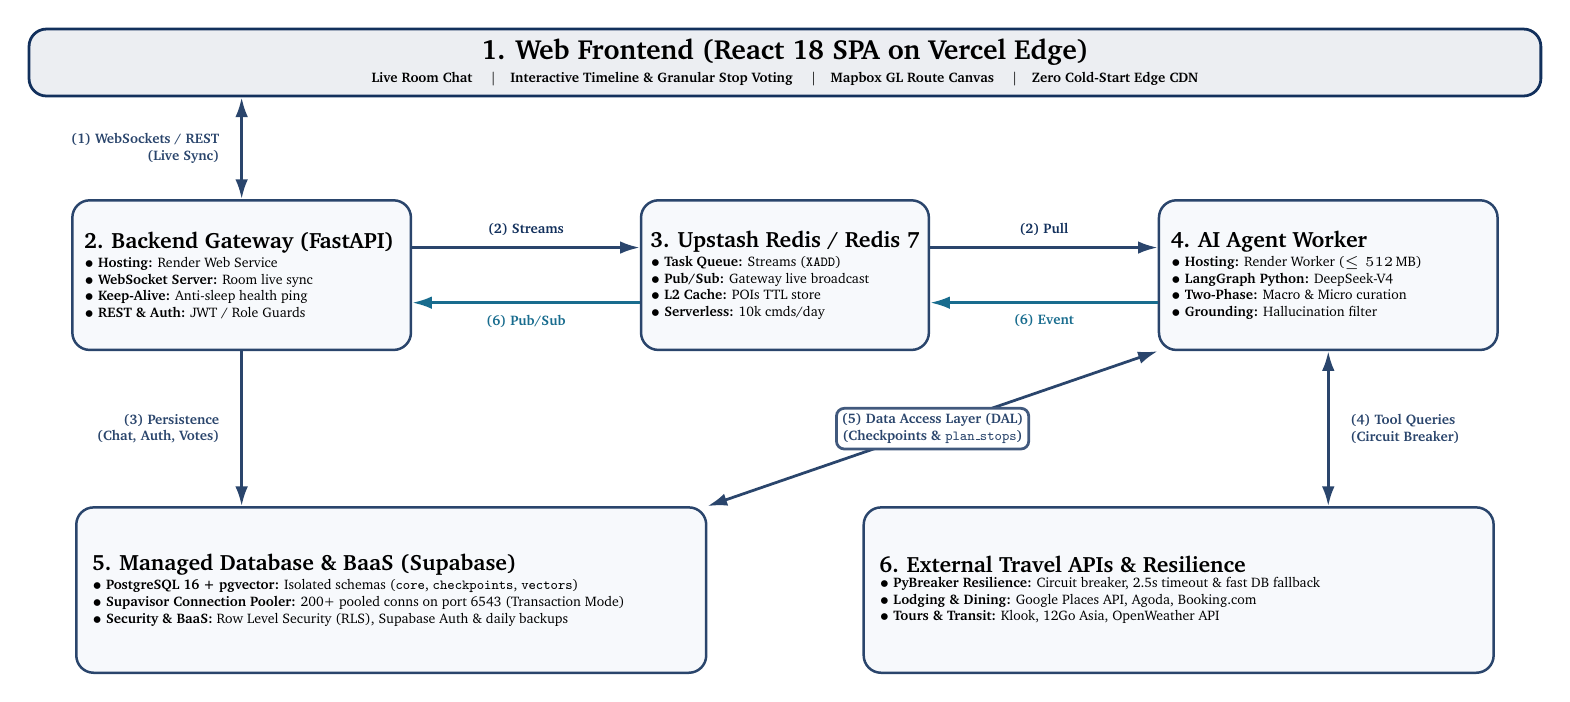
\begin{tikzpicture}[
  layerbox/.style={rectangle, draw=primaryblue!90, fill=subtlegray, rounded corners=2.2mm, line width=0.9pt, minimum width=4.3cm, minimum height=1.9cm, align=left, font=\scriptsize},
  topbox/.style={rectangle, draw=primaryblue, fill=primaryblue!8!white, rounded corners=2.2mm, line width=1.0pt, minimum width=19.2cm, minimum height=0.85cm, align=center, font=\scriptsize},
  widebox/.style={rectangle, draw=primaryblue!90, fill=subtlegray, rounded corners=2.2mm, line width=0.9pt, minimum width=8.0cm, minimum height=2.1cm, align=left, font=\scriptsize},
  flowarrow/.style={-{Latex[length=2.5mm,width=1.6mm]}, line width=1.0pt, color=primaryblue!90},
  biarrow/.style={{Latex[length=2.5mm,width=1.6mm]}-{Latex[length=2.5mm,width=1.6mm]}, line width=1.0pt, color=primaryblue!90}
]

% Top: Frontend SPA Banner
\node[topbox] (fe) at (0, 4.6) {
\textbf{\normalsize 1. Web Frontend (React 18 SPA on Vercel Edge)}\\[0.02cm]
\parbox{18.6cm}{\centering \tiny
\textbf{Live Room Chat} \quad$\vert$\quad
\textbf{Interactive Timeline \& Granular Stop Voting} \quad$\vert$\quad
\textbf{Mapbox GL Route Canvas} \quad$\vert$\quad
\textbf{Zero Cold-Start Edge CDN}
}
};

% Middle Row: Gateway, Redis, AI Agent
\node[layerbox] (be) at (-6.9, 1.9) {
\textbf{\footnotesize 2. Backend Gateway (FastAPI)}\\[0.02cm]
\parbox{4.0cm}{\raggedright \tiny
$\bullet$ \textbf{Hosting:} Render Web Service\\
$\bullet$ \textbf{WebSocket Server:} Room live sync\\
$\bullet$ \textbf{Keep-Alive:} Anti-sleep health ping\\
$\bullet$ \textbf{REST \& Auth:} JWT / Role Guards
}
};

\node[layerbox, minimum width=3.5cm] (redis) at (0, 1.9) {
\textbf{\footnotesize 3. Upstash Redis / Redis 7}\\[0.02cm]
\parbox{3.2cm}{\raggedright \tiny
$\bullet$ \textbf{Task Queue:} Streams (\texttt{XADD})\\
$\bullet$ \textbf{Pub/Sub:} Gateway live broadcast\\
$\bullet$ \textbf{L2 Cache:} POIs TTL store\\
$\bullet$ \textbf{Serverless:} 10k cmds/day
}
};

\node[layerbox] (ai) at (6.9, 1.9) {
\textbf{\footnotesize 4. AI Agent Worker}\\[0.02cm]
\parbox{4.0cm}{\raggedright \tiny
$\bullet$ \textbf{Hosting:} Render Worker ($\le 512$\,MB)\\
$\bullet$ \textbf{LangGraph Python:} DeepSeek-V4\\
$\bullet$ \textbf{Two-Phase:} Macro \& Micro curation\\
$\bullet$ \textbf{Grounding:} Hallucination filter
}
};

% Bottom Row: Database and External Travel APIs
\node[widebox] (db) at (-5.0, -2.1) {
\textbf{\footnotesize 5. Managed Database \& BaaS (Supabase)}\\[0.02cm]
\parbox{7.6cm}{\raggedright \tiny
$\bullet$ \textbf{PostgreSQL 16 + pgvector:} Isolated schemas (\texttt{core}, \texttt{checkpoints}, \texttt{vectors})\\
$\bullet$ \textbf{Supavisor Connection Pooler:} 200+ pooled conns on port 6543 (Transaction Mode)\\
$\bullet$ \textbf{Security \& BaaS:} Row Level Security (RLS), Supabase Auth \& daily backups
}
};

\node[widebox] (ext) at (5.0, -2.1) {
\textbf{\footnotesize 6. External Travel APIs \& Resilience}\\[0.02cm]
\parbox{7.6cm}{\raggedright \tiny
$\bullet$ \textbf{PyBreaker Resilience:} Circuit breaker, 2.5s timeout \& fast DB fallback\\
$\bullet$ \textbf{Lodging \& Dining:} Google Places API, Agoda, Booking.com\\
$\bullet$ \textbf{Tours \& Transit:} Klook, 12Go Asia, OpenWeather API
}
};

% Connectors
\draw[biarrow] (be.north) -- (be.north |- fe.south) node[midway, left=0.15cm, font=\tiny\bfseries, align=right]{\textbf{(1)} WebSockets / REST\\(Live Sync)};
\draw[flowarrow] ($(be.east)+(0, 0.35)$) -- ($(redis.west)+(0, 0.35)$) node[midway, above=0.02cm, font=\tiny\bfseries, text=primaryblue]{\textbf{(2)} Streams};
\draw[flowarrow] ($(redis.east)+(0, 0.35)$) -- ($(ai.west)+(0, 0.35)$) node[midway, above=0.02cm, font=\tiny\bfseries, text=primaryblue]{\textbf{(2)} Pull};
\draw[flowarrow, color=accentteal] ($(ai.west)-(0, 0.35)$) -- ($(redis.east)-(0, 0.35)$) node[midway, below=0.02cm, font=\tiny\bfseries, text=accentteal]{\textbf{(6)} Event};
\draw[flowarrow, color=accentteal] ($(redis.west)-(0, 0.35)$) -- ($(be.east)-(0, 0.35)$) node[midway, below=0.02cm, font=\tiny\bfseries, text=accentteal]{\textbf{(6)} Pub/Sub};
\draw[flowarrow] (be.south) -- (be.south |- db.north) node[midway, left=0.15cm, font=\tiny\bfseries, align=right]{\textbf{(3)} Persistence\\(Chat, Auth, Votes)};
\draw[biarrow] (ai.south) -- (ai.south |- ext.north) node[midway, right=0.15cm, font=\tiny\bfseries, align=left]{\textbf{(4)} Tool Queries\\(Circuit Breaker)};
\draw[biarrow] (ai.south west) -- (db.north east) node[midway, font=\tiny\bfseries, fill=white, draw=primaryblue!80, rounded corners=1.0mm, inner sep=2.0pt, align=center]{\textbf{(5)} Data Access Layer (DAL)\\(Checkpoints \& \texttt{plan\_stops})};

\end{tikzpicture}
}
\vspace{-0.25cm}
\caption{TripMate AI system architecture: component layers, cloud providers, and operational interfaces (1)--(6)}
\label{fig:system_flow}
\end{figure}

\subsection{Technology Stack}
\begin{table}[H]
\centering
\footnotesize
\renewcommand{\arraystretch}{1.05}
\begin{tabularx}{\textwidth}{@{}l p{3.2cm} p{3.0cm} X@{}}
\toprule
\textbf{Tier} & \textbf{Core Technology} & \textbf{Cloud Platform} & \textbf{Architectural Role} \\
\midrule
\textbf{Frontend} & React 18 + TypeScript & \textbf{Vercel} & Interactive timeline, collaborative voting cards, Mapbox GL canvas on Edge CDN. \\
\midrule
\textbf{Backend Gateway} & FastAPI (Python 3.11+) & \textbf{Render.com} & REST endpoints, WebSocket room server, anti-sleep keep-alive pings. \\
\midrule
\textbf{AI Agent Layer} & LangGraph Python & \textbf{Render.com} & Unified DeepSeek-V4 agent, two-phase states, memory bounded $\le 280$\,MB. \\
& Model Abstraction & Cloud LLM APIs & Primary: DeepSeek-V4; Fallback: OpenAI GPT-4o, Claude, Gemini. \\
\midrule
\textbf{Database \& Auth} & PostgreSQL 16 + \texttt{pgvector} & \textbf{Supabase} & Relational persistence, Supavisor connection pooler (port 6543), RLS security. \\
\midrule
\textbf{Queue \& Cache} & Redis 7 / Redis Streams & \textbf{Upstash Redis} & Asynchronous task broker, WebSocket Pub/Sub broadcast, 24h TTL POI cache. \\
\midrule
\textbf{Resilience \& Ops} & PyBreaker / OpenTelemetry & Cloud Observability & External API circuit breakers (2.5s timeout), distributed tracing, LangSmith. \\
\bottomrule
\end{tabularx}
\vspace{-0.2cm}
\caption{Core technology stack and cloud platform distribution for TripMate AI}
\label{tab:tech_stack}
\end{table}

\subsection{Cloud Deployment Architecture (Vercel, Supabase, Render)}
\label{sec:deployment_architecture}
TripMate AI is deployed across modern cloud platforms (Vercel, Supabase, Render) configured for high availability:
\begin{itemize}
\item \textbf{Frontend (Vercel):} React 18 SPA hosted on Vercel's Global Edge CDN with zero cold-start latency, automatic GitHub CI/CD, and custom domain SSL.
\item \textbf{Backend Gateway \& AI Worker (Render):} FastAPI ASGI application and LangGraph worker running in containerized environments (512\,MB RAM). An automated keep-alive cron ping to \texttt{/api/healthz} prevents instance idling during active planning sessions.
\item \textbf{Database \& Auth (Supabase):} Managed PostgreSQL 16 with \texttt{pgvector} and Supabase Auth. The built-in Supavisor connection pooler (port 6543, Transaction Mode) multiplexes 200+ client sessions across 15 physical connections, maintaining high connection availability.
\item \textbf{Task Queue \& Cache (Upstash Redis):} Serverless Redis managing Redis Streams for asynchronous AI agent task dispatch and Redis Pub/Sub for live room WebSocket broadcasting.
\end{itemize}

\clearpage
% ==========================================
% PAGE 4: END-TO-END OPERATIONAL FLOW & SEQUENCE EXECUTION
% ==========================================
\subsection{End-to-End Operational Flow}
\label{sec:system_flow}
Figure~\ref{fig:operational_flow_diagram} visualizes the operational execution lifecycle of interfaces \textbf{(1)--(6)} from the System Architecture (Figure~\ref{fig:system_flow}) as an end-to-end UML sequence diagram, showing the asynchronous decoupling of client interactions on Vercel, background AI processing on Render, resilient tool execution, and real-time room broadcasting. Table~\ref{tab:system_flow_summary} summarizes each operational stage, execution mode, and dependent triggers.

\begin{figure}[H]
\centering
\resizebox{0.95\textwidth}{!}{
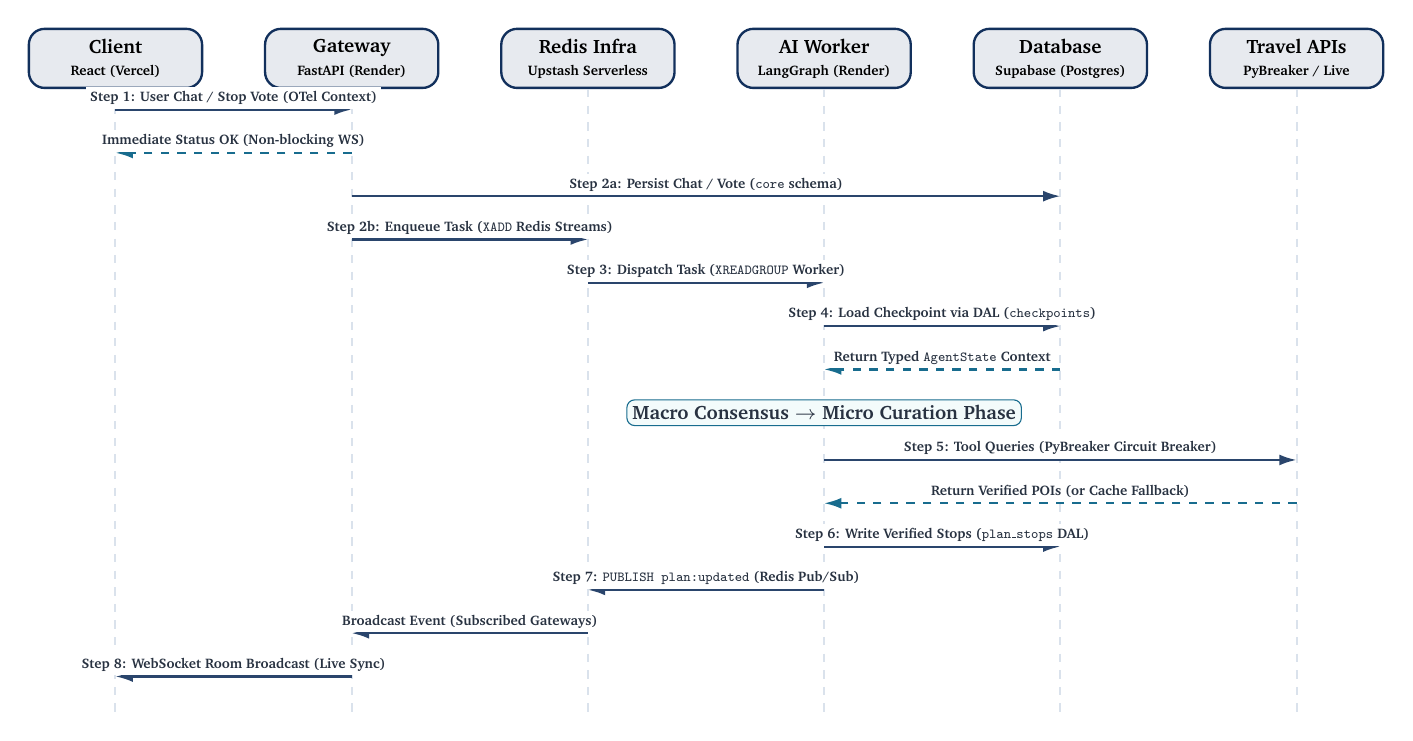
\begin{tikzpicture}[
  participant/.style={rectangle, draw=primaryblue, fill=primaryblue!10!white, rounded corners=2mm, line width=0.85pt, minimum width=2.2cm, minimum height=0.75cm, align=center, font=\scriptsize\bfseries},
  seqarrow/.style={-{Latex[length=2.2mm,width=1.4mm]}, line width=0.85pt, color=primaryblue!90},
  retarrow/.style={-{Latex[length=2.2mm,width=1.4mm]}, dashed, line width=0.8pt, color=accentteal},
  lbl/.style={font=\tiny\bfseries, fill=white, inner sep=1.5pt, text=darkcharcoal}
]

% 6 Lifelines Spaced Exactly 3.0cm Apart Across 15.0cm
\node[participant] (c) at (0, 0) {Client\\{\tiny React (Vercel)}};
\node[participant] (gw) at (3.0, 0) {Gateway\\{\tiny FastAPI (Render)}};
\node[participant] (q) at (6.0, 0) {Redis Infra\\{\tiny Upstash Serverless}};
\node[participant] (ai) at (9.0, 0) {AI Worker\\{\tiny LangGraph (Render)}};
\node[participant] (db) at (12.0, 0) {Database\\{\tiny Supabase (Postgres)}};
\node[participant] (ext) at (15.0, 0) {Travel APIs\\{\tiny PyBreaker / Live}};

% Vertical Lifelines
\draw[dashed, color=bordergray, line width=0.7pt] (c.south) -- (0, -8.3);
\draw[dashed, color=bordergray, line width=0.7pt] (gw.south) -- (3.0, -8.3);
\draw[dashed, color=bordergray, line width=0.7pt] (q.south) -- (6.0, -8.3);
\draw[dashed, color=bordergray, line width=0.7pt] (ai.south) -- (9.0, -8.3);
\draw[dashed, color=bordergray, line width=0.7pt] (db.south) -- (12.0, -8.3);
\draw[dashed, color=bordergray, line width=0.7pt] (ext.south) -- (15.0, -8.3);

% Step 1: User Action
\draw[seqarrow] (0, -0.65) -- (3.0, -0.65);
\node[lbl] at (1.5, -0.50) {\textbf{Step 1:} User Chat / Stop Vote (OTel Context)};

% Immediate Non-Blocking Ack
\draw[retarrow] (3.0, -1.20) -- (0, -1.20);
\node[lbl] at (1.5, -1.05) {Immediate Status OK (Non-blocking WS)};

% Step 2a: Persist Chat / Votes
\draw[seqarrow] (3.0, -1.75) -- (12.0, -1.75);
\node[lbl] at (7.5, -1.60) {\textbf{Step 2a:} Persist Chat / Vote (\texttt{core} schema)};

% Step 2b: Enqueue Task
\draw[seqarrow] (3.0, -2.30) -- (6.0, -2.30);
\node[lbl] at (4.5, -2.15) {\textbf{Step 2b:} Enqueue Task (\texttt{XADD} Redis Streams)};

% Step 3: Dispatch Task
\draw[seqarrow] (6.0, -2.85) -- (9.0, -2.85);
\node[lbl] at (7.5, -2.70) {\textbf{Step 3:} Dispatch Task (\texttt{XREADGROUP} Worker)};

% Step 4: Load Checkpoint via DAL
\draw[seqarrow] (9.0, -3.40) -- (12.0, -3.40);
\node[lbl] at (10.5, -3.25) {\textbf{Step 4:} Load Checkpoint via DAL (\texttt{checkpoints})};

\draw[retarrow] (12.0, -3.95) -- (9.0, -3.95);
\node[lbl] at (10.5, -3.80) {Return Typed \texttt{AgentState} Context};

% Internal State Transition Node
\node[lbl, fill=badgeteal!40!white, draw=accentteal, rounded corners=1mm, inner sep=2pt] at (9.0, -4.50) {\scriptsize Macro Consensus $\rightarrow$ Micro Curation Phase};

% Step 5: Resilient Tool Queries
\draw[seqarrow] (9.0, -5.10) -- (15.0, -5.10);
\node[lbl] at (12.0, -4.95) {\textbf{Step 5:} Tool Queries (PyBreaker Circuit Breaker)};

\draw[retarrow] (15.0, -5.65) -- (9.0, -5.65);
\node[lbl] at (12.0, -5.50) {Return Verified POIs (or Cache Fallback)};

% Step 6: Persist Stops via DAL
\draw[seqarrow] (9.0, -6.20) -- (12.0, -6.20);
\node[lbl] at (10.5, -6.05) {\textbf{Step 6:} Write Verified Stops (\texttt{plan\_stops} DAL)};

% Step 7: Publish Plan Event
\draw[seqarrow] (9.0, -6.75) -- (6.0, -6.75);
\node[lbl] at (7.5, -6.60) {\textbf{Step 7:} \texttt{PUBLISH plan:updated} (Redis Pub/Sub)};

% Step 7b: Multi-Instance Broadcast
\draw[seqarrow] (6.0, -7.30) -- (3.0, -7.30);
\node[lbl] at (4.5, -7.15) {Broadcast Event (Subscribed Gateways)};

% Step 8: WebSocket Broadcast
\draw[seqarrow] (3.0, -7.85) -- (0, -7.85);
\node[lbl] at (1.5, -7.70) {\textbf{Step 8:} WebSocket Room Broadcast (Live Sync)};

\end{tikzpicture}
}
\vspace{-0.25cm}
\caption{UML sequence diagram: end-to-end operational execution flow for the unified TripMate AI Agent}
\label{fig:operational_flow_diagram}
\end{figure}

\begin{table}[H]
\centering
\footnotesize
\renewcommand{\arraystretch}{1.06}
\begin{tabularx}{\textwidth}{@{}c l c l >{\raggedright\arraybackslash}X@{}}
\toprule
\textbf{Step} & \textbf{Interface Path} & \textbf{Mode} & \textbf{Depends On} & \textbf{Operational Function} \\
\midrule
\textbf{1} & \textbf{(1)} Frontend $\rightarrow$ Gateway & Sync & User action & Transmits chat message or stop vote payload with OpenTelemetry context. \\
\textbf{2a} & \textbf{(3)} Gateway $\rightarrow$ Database & Sync & Step 1 & Persists chat logs and vote counts into Supabase (\texttt{core} schema). \\
\textbf{2b} & \textbf{(2)} Gateway $\rightarrow$ Redis (Streams) & Async & Step 1 & Dispatches non-blocking task to Redis Streams (\texttt{XADD}); returns immediate HTTP/WS ack. \\
\textbf{3} & \textbf{(2)} Redis (Streams) $\rightarrow$ AI Agent & Async & Step 2b & LangGraph worker consumes task via \texttt{XREADGROUP} consumer group. \\
\textbf{4} & \textbf{(5)} AI Agent $\leftarrow$ Database & Async & Step 3 & Loads active session checkpoint and context via DAL from \texttt{checkpoints} schema. \\
\textbf{4b} & LangGraph State Transition & Internal & Step 4 & Evaluates consensus and transitions between Macro Planning and Micro Curation phases. \\
\textbf{5} & \textbf{(4)} AI Agent $\leftrightarrow$ Travel APIs & Parallel & Step 4b & Queries live APIs via PyBreaker circuit breaker; falls back to cache/vector gems on timeout. \\
\textbf{6} & \textbf{(5)} AI Agent $\rightarrow$ Database & Async & Step 5 & Writes normalized, verified venue records to \texttt{plan\_stops} via DAL. \\
\textbf{7} & \textbf{(6)} AI Agent $\rightarrow$ Redis $\rightarrow$ Gateway & Async & Step 6 & Publishes \texttt{plan:updated} via Redis Pub/Sub to synchronize all FastAPI gateway instances. \\
\textbf{8} & \textbf{(1)} Gateway $\rightarrow$ Frontend & Push & Step 7 & Broadcasts refreshed itinerary to all connected room members via WebSockets. \\
\bottomrule
\end{tabularx}
\vspace{-0.2cm}
\caption{Unified AI Agent operational execution flow mapped to system interfaces}
\label{tab:system_flow_summary}
\end{table}

\textbf{Dynamic On-the-Go Adaptability:} When conditions change unexpectedly (e.g., sudden rain), a member chats: \textit{``it is raining, find an indoor cafe nearby''}. FastAPI immediately returns an acknowledgment (non-blocking WebSocket), records the message in Supabase (\texttt{core} schema, Step 2a), and enqueues an asynchronous task to Redis Streams (Step 2b). The LangGraph AI Agent worker consumes the task (Step 3), restores the active session checkpoint from Supabase via DAL (Step 4), transitions directly to its Micro Curation state (Step 4b), queries nearby indoor venues in parallel through the resilient PyBreaker-guarded API and cache layer (Step 5), modifies \textbf{only the affected single row in \texttt{plan\_stops}} in PostgreSQL (Step 6), publishes the update event to Redis Pub/Sub (Step 7), and FastAPI broadcasts the updated stop to all room members via WebSockets (Step 8).

\clearpage
% ==========================================
% PAGE 5: NFRs, LATENCY BUDGET, CAPACITY, SECURITY & CONCLUSION (CONTINUOUS FLOW)
% ==========================================
\section{System Targets, Evaluation \& Engineering Foundations}
\label{sec:nfr}

\subsection{Core System Targets: Latency, Capacity, Evaluation \& Planet-Scale Scaling}
\label{sec:system_targets}
\label{sec:latency_budget}
\label{sec:capacity_concurrency}

TripMate AI defines four concrete, measurable performance targets:

\begin{itemize}[leftmargin=1.2em]
\item \textbf{Latency Targets:}
  \begin{itemize}[leftmargin=1.0em]
  \item \textit{User Actions:} $< 80$\,ms WebSocket ACK for chat messages and votes.
  \item \textit{Initial AI Response (TTFT):} $< 800$\,ms token streaming so users see answers immediately instead of waiting on a blank screen.
  \item \textit{Full Answer Times:} $6$--$12$\,s for macro roadmaps; $10$--$20$\,s for micro venue grounding; $3$--$6$\,s for 1-click swaps (Table~\ref{tab:latency_budget}).
  \end{itemize}
\item \textbf{Capacity Targets:}
  \begin{itemize}[leftmargin=1.0em]
  \item \textit{Concurrency:} 50--100 Concurrent Active Users (CCU) across 10--20 active rooms (3--6 users/room).
  \item \textit{Throughput:} 150--250 req/s on FastAPI gateway; 5--8 concurrent AI jobs with Redis queue buffer.
  \item \textit{Storage \& Connections:} 30,000+ saved trips in PostgreSQL; 200+ user sessions multiplexed into 15 database connections via Supavisor pooler.
  \end{itemize}
\item \textbf{Evaluation Targets (Success Criteria):}
  \begin{itemize}[leftmargin=1.0em]
  \item \textit{AI Accuracy:} $\ge 98\%$ venues verified on Google Places ($0\%$ fake places); $\ge 95\%$ adherence to budget and distance constraints ($\le 2.5$\,km).
  \item \textit{Consensus Speed:} Reduce group decision time from 2--3 days down to $< 15$ minutes; $\ge 85\%$ initial stop approval.
  \item \textit{System Health:} $\ge 99.5\%$ uptime; $< 100$\,ms multi-user WebSocket synchronization delay.
  \end{itemize}
\item \textbf{Planet-Scale Scalability Targets:}
  \begin{itemize}[leftmargin=1.0em]
  \item Designed to scale globally without architectural rewrites: Vercel Global Edge CDN for sub-100\,ms frontend delivery worldwide, stateless FastAPI and LangGraph workers on Render that scale horizontally, Redis Streams for queue buffering, and Supavisor connection pooling for database scalability.
  \end{itemize}
\end{itemize}

\begin{table}[H]
\centering
\footnotesize
\renewcommand{\arraystretch}{1.06}
\begin{tabularx}{\textwidth}{@{}l c c >{\raggedright\arraybackslash}X@{}}
\toprule
\textbf{Interaction Type} & \textbf{TTFT} & \textbf{Full Time} & \textbf{Operational Context} \\
\midrule
\textbf{Member Action / Vote} & $< 80$\,ms & $< 80$\,ms & Instant WebSocket ACK with atomic database update. \\
\textbf{Quick Clarification / Q\&A} & $< 600$\,ms & $3$--$5$\,s & Direct LLM response for dietary, parking, or hours queries. \\
\textbf{Macro Itinerary Drafting} & $< 800$\,ms & $6$--$12$\,s & LangGraph Phase 1 themes and multi-day pacing roadmap. \\
\textbf{Micro Spot Grounding} & $< 1.0$\,s & $10$--$20$\,s & Parallel Google Places checks and route matrix calculation. \\
\textbf{1-Click Swap / Revision} & $< 500$\,ms & $3$--$6$\,s & Instant replacement with pre-verified backup venue. \\
\bottomrule
\end{tabularx}
\vspace{-0.2cm}
\caption{TripMate AI multi-turn interaction latency budget and response times}
\label{tab:latency_budget}
\end{table}

\subsection{Evaluation Methodology: Verifying Agent \& System Effectiveness}
\label{sec:evaluation}

To empirically verify performance, TripMate AI evaluates both the AI Agent and the cloud System against concrete benchmarks:

\subsubsection{AI Agent Evaluation (Planning Quality \& Accuracy)}
\begin{itemize}[leftmargin=1.2em]
\item \textbf{Grounding \& Hallucination Test:} 100 automated test prompts across multiple cities check every venue against Google Places API.
\textbf{Metric:} Verification Rate $= (\text{Verified POIs with Place ID} / \text{Total POIs}) \ge 98\%$; $0\%$ fake POIs.
\item \textbf{Constraint Satisfaction Test:} Scripts verify that generated stops match budget limits, dietary preferences, and spatial clustering ($\le 2.5$\,km radius, $\le 20$\,min transit).
\textbf{Metric:} $\ge 95\%$ constraint pass rate.
\item \textbf{User Acceptance \& Speed Test:} Pilot trials with 10 real user groups (3--6 members) track voting telemetry and time to plan completion.
\textbf{Metric:} $\ge 85\%$ first-recommendation approval; consensus reached in $< 15$ minutes.
\end{itemize}

\subsubsection{System Performance Evaluation (Infrastructure \& Reliability)}
\begin{itemize}[leftmargin=1.2em]
\item \textbf{Latency \& Tracing Test:} OpenTelemetry and LangSmith track end-to-end timing across Gateway $\rightarrow$ Queue $\rightarrow$ Agent $\rightarrow$ DB $\rightarrow$ WebSocket.
\textbf{Metric:} TTFT $< 800$\,ms, action ACK $< 80$\,ms, room sync $< 100$\,ms.
\item \textbf{Load \& Concurrency Stress Test:} Locust/k6 simulates 50--100 CCU in 10--20 rooms chatting, voting, and generating itineraries simultaneously.
\textbf{Metric:} Sustained 150--250 req/s, error rate $< 0.5\%$, worker memory $\le 512$\,MB.
\item \textbf{Fault Tolerance Test:} Chaos testing introduces 5s API delays and simulates primary LLM API outages.
\textbf{Metric:} PyBreaker trips in 2.5s to return cached POIs; seamless fallback to secondary LLMs (GPT-4o/Gemini) without session drop.
\end{itemize}

\subsection{Security, Multi-Tenant Privacy \& Reliability}
\label{sec:security_nfr}
\begin{itemize}[leftmargin=1.2em]
\item \textbf{Data Privacy (Supabase RLS):} Database-level policies ensure users only access data in their own planning rooms.
\item \textbf{Atomic Voting:} Atomic SQL updates and Redis counters prevent race conditions when multiple members vote simultaneously.
\item \textbf{Input Sanitization:} Chat inputs are sanitized before LLM processing to prevent prompt injection attempts.
\item \textbf{Session Recovery:} LangGraph execution checkpoints are saved in PostgreSQL, enabling instant recovery if a container restarts.
\end{itemize}

\section{Expected Impact \& Conclusion}
\label{sec:conclusion}
TripMate AI represents a paradigm shift in collaborative group planning by unifying conversational AI intelligence, deterministic grounding, and modern web collaboration into a cohesive, scalable production system:
\begin{itemize}
\item \textbf{Sub-15-Minute Consensus:} Compresses days of scattered group chat debates into a structured, real-time 15-minute consensus session, eliminating organizer fatigue.
\item \textbf{Zero-Hallucination Guarantee:} Grounded in physical reality via the Four-Tier Grounding Pipeline, strictly validating place IDs, operational status, opening hours, and geographic proximity against live travel APIs.
\item \textbf{Production-Grade Cloud Performance:} Demonstrates exceptional engineering feasibility by orchestrating Vercel, Render, and Supabase while maintaining sub-800\,ms initial response streaming and robust 50--100 CCU concurrency.
\item \textbf{Enterprise-Grade Security \& Resilience:} Enforces database-level isolation via Supabase RLS, atomic concurrency control for voting, and seamless checkpoint recovery for uncompromised data integrity.
\item \textbf{Living, Adaptive Itineraries:} Couples transactional relational persistence with dynamic on-trip adaptation, allowing groups to modify single stops on the fly without recalculating untouched itinerary blocks.
\end{itemize}

\vspace{0.25cm}
\begin{center}
\small\color{primaryblue}\textbf{\textit{TripMate AI turns group trip planning from an exhausting chore into an effortless, collaborative, and mathematically grounded experience.}}
\end{center}

\end{document}
